\section{Analyse}

\subsection{Messaufbau}

Um die verschiedenen Implementationen zu testen, wird ein Benchmark genutzt. In diesem Benchmark werden über eine Funktion eine bestimmte Menge an Elementen, in diesem Falle Nachrichten mit drei Elementen - der Nachrichtennummer, dem Text 'Dummy' und einem Timestamp - gesendet und empfangen. Der Ablauf des \textit{Client-Server-Systems} kann unter verschiedenen Bedingungen simuliert werden. 
So kann die Liste mit welchem die \textit{Holdback Queue} gefüllt wird unterschiedliche Vorsortierungen haben. Damit können die interne Heap und List Struktur verglichen werden.
Die Zeit zum Senden und Empfangen der Eingabelisten wird in einer csv-Datei für verschiedene Listengrößen gespeichert und nach Abschluss der Messung über die Python \textit{matplotlib} Library geplottet.
Die Schrittgröße zum Vergrößern und die Sortierung der Eingabelisten, die Anzahl der Startelemente, die der Schritte und die übergebenen \textit{Holdback Queues} sind parametrisiert. So können in einem Plot auch mehrere Implementierungen miteinander verglichen werden. An der y-Achse ist die Zeit des Sende-Empfangs-Prozesses in Millisekunden pro Element und an der x-Achse die Größe der Eingabeliste dargestellt. 
Eine weitere Funktion des Benchmarks ist das Erzeugen einer Eingabeliste, anhand welcher die aus der Aufgabenstellung hervorgehende reale Bedingung simuliert werden kann. Diese Sortierung wird im Folgenden als reale Sortierung bezeichnet. Die Elemente werden hierbei so sortiert, wie sie von dem \textit{Client System} an den \textit{Server}, beziehungsweise von dem Server an die Holdback Queue gesendet werden. Die Reihenfolge der Nachrichtennummern ist annähernd aufsteigend also ähnlich zu einer linearen Trendlinie mit hoher Wertestreuung. 
Das Limit der Delivery Queue wird dynamisch erhöht und ergibt sich aus $DLQLimit = ceil(InputVal * length(Eingabeliste) / 100)$. Die Variable \textit{InputVal} hat als Defaultwert 100, kann im Benchmark aber auch verändert werden. Bei Default Einstellungen ist das Limit der Delivery Queue also immer gleich der Größe der Eingabeliste. 
Analysiert werden die zwei \textit{Holdback Queue} Strukturen unter verschiedenen Bedingungen und außerdem die Implementierungen mit und ohne \textit{Pattern Matching}. 
Die Startgröße der Liste wird im Folgenden 100 sein, die Schrittgröße liegt bei 100 und die Anzahl der Schritte ist entweder 100 oder 250.

\subsection{Messergebnisse}

Der Plot aus Abbildung \ref{fig:auf_hbq_pattern} zeigt die Messergebnisse des Benchmarks der \textit{Holdback Queue} mit und ohne \textit{Pattern Matching} im Vergleich. Die orange Trendlinie und die blauen Punkte gehören zur \textit{Holdback Queue} mit \textit{Pattern Matching}. Gemessen wurde mit 100 Schritten, die zuletzt übergebene Liste enthielt also 10100 Elemente. Die Nachrichten in der Liste waren aufsteigend sortiert. Auffällig ist, dass sich die Messungen kaum unterscheiden. Die Trendlinien sind beide linear und scheinen nahezu identisch zu sein. Auch die Streuung der Messwerte um diese Trendlinien ist sehr gering. Die Dauer des Senden und Empfangens von 10000 Elementen beträgt 0,24ms pro Element.

\begin{figure}[htbp]
\begin{center}
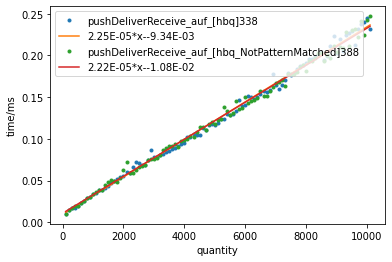
\includegraphics[scale=0.7]{Latex/Bilder/Plots/auf_hbq_patternMatching.png}
\caption{\label{fig:auf_hbq_pattern} aufsteigend - vgl. Heap (mit und ohne Pattern-Matching)} 
\end{center}
\end{figure}

\newpage
In dem Plot aus Abbildung \ref{fig:auf_heapList} ist der Vergleich der \textit{Holdback Queue} implementiert mit interner Liste und mit internem Heap gezeigt. Gemessen wurde mit 100 Schritten, die Sortierung der Elemente ist wieder aufsteigend. Die orange Linie und die blauen Punkte gehören wieder zu dem Heap. Dessen Messwerte sind sehr ähnlich zu den Messwerten des oberen Plots. Allerdings gilt das auch für die List Messwerte. Die Streuung ist hier etwas größer, allerdings immer noch sehr gering und voraussichtlich eher Hintergrundprozessen des Betriebssystems während der Messdurchführung geschuldet. Die Trendlinien sind somit auch wieder linear. Hier dauert der Prozess bei 10000 Elementen wie bei der letzten Messung 0,24ms pro Element. 

\begin{figure}[htbp]
\begin{center}
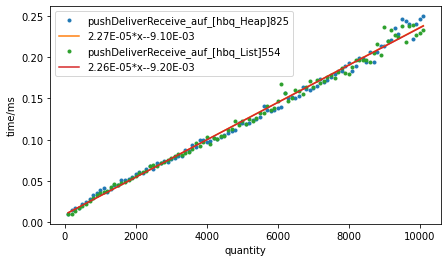
\includegraphics[scale=0.7]{Latex/Bilder/Plots/auf_HBQ_HeapList.png}
\caption{\label{fig:auf_heapList} aufsteigend - vgl. Heap, List} 
\end{center}
\end{figure}

Dieser Plot (Abbildung \ref{fig:rand_heapList}) zeigt die Messungen der zwei verschiedenen \textit{Holdback Queue} Strukturen bei zufällig sortierter Liste mit 100 Schritten. Im Vergleich zu den letzten beiden Plots ist hier ein deutlicher Unterschied zwischen den beiden Messungen zu erkennen. Die rote Trendlinie und die grünen Punkte sind dem Heap zugeordnet. Dieser liegt bei 10000 Elementen in der Eingabeliste bei 0,175ms pro Element, die Liste benötigt 0,225ms. Das ergibt eine Differenz von 0,05ms bei 10000 Elementen. Außerdem ist auffällig, dass die Messungen bei zufälliger Eingabeliste um mindestens 0,015ms schneller ist. Der Verlauf beider Messungen ist linear, allerdings ist die Streuung der Werte in der Messung für die Liste deutlich höher. Bedingt kann dies aber auch daran liegen, dass die Eingabeliste immer zufällig sortiert ist. Durch die Implementierung der \textit{Holdback Queue} als Liste ist die Sortierung einer eher aufsteigenden Liste deutlich schneller als die einer eher absteigend sortierten. 

\begin{figure}[htbp]
\begin{center}
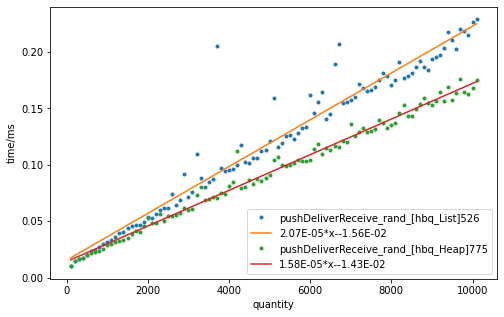
\includegraphics[scale=0.525]{Latex/Bilder/Plots/rand_Heap_List.png}
\caption{\label{fig:rand_heapList} random - vgl. Heap, List} 
\end{center}
\end{figure}

Im Plot aus Abbildung \ref{fig:real_heapList} werden die Messungen der \textit{Holdback Queue} mit internem Heap und mit interner Liste bei realer Sortierung gezeigt. Die Trendlinien sind wieder nahezu identisch und die Streuung der Werte ist sehr gering, nimmt aber bei steigenden Elementen zu. Das Senden und Empfangen von 10000 Elementen dauert 0,27ms pro Element.

\begin{figure}[htbp]
\begin{center}
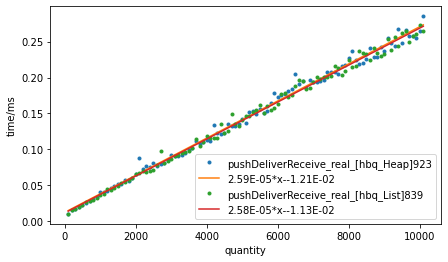
\includegraphics[scale=0.625]{Latex/Bilder/Plots/real_hbq_Heap_List.png}
\caption{\label{fig:real_heapList} real - vgl. Heap, List} 
\end{center}
\end{figure}

Im nächsten Plot (Abbildung \ref{fig:real_hbqAll}) sind die Messungen der drei verschiedenen \textit{Holdback Queues} (interner Heap, interne Liste und kein \textit{Pattern Matching}) mit 250 Schritten dargestellt. Im letzten Durchlauf wurden hier also 25100 Elemente in die \textit{Holdback Queue} eingefügt. Der Benchmark wurde unter realen Bedingungen simuliert. Der Verlauf der Trendlinien ist linear und die, der drei verschiedenen Implementierungen, liegen sehr nah beieinander. Bei 25000 Elementen in der Eingabeliste ist in dieser Messung die \textit{Holdback Queue} mit interner Liste mit 0,68ms pro Element am schnellsten, danach folgt die Queue mit internem Heap, aber ohne \textit{Pattern Matching}, mit 0,74ms und danach die \textit{Holdback Queue} mit internem Heap und \textit{Pattern Matching}. Diese hat eine benötigte Dauer von 0,76ms. Die Streuung der Werte ist zu Beginn sehr gering und wird bei steigender Größe immer höher.

\begin{figure}[htbp]
\begin{center}
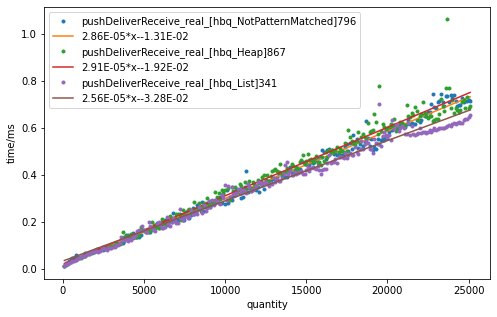
\includegraphics[scale=0.6]{Latex/Bilder/Plots/real_hbq.png}
\caption{\label{fig:real_hbqAll} real - vgl. List, Heap (mit und ohne Pattern-Matching)} 
\end{center}
\end{figure}

Im Plot aus Abbildung \ref{fig:real_heapListPercent} werden die \textit{Holdback Queues} mit interner Liste und Heap jeweils mit verschiedenen \textit{Delivery Queue} Limits initialisiert. Diese \textit{Delivery Queue} Limits entsprechen 1\% und 10\% der übergebenen Eingabeliste. Zu Beobachten ist, dass die \textit{Holdback Queues} mit kleineren \textit{Delivery Queue} Limits fast um das 5-fache schneller sind. Die Trendlinien der beiden Queues mit 1\% sind fast identisch, die \textit{Holdback Queue} mit internem Heap (blaue Werte) beendet den Prozess bei 10\% etwas schneller als die mit interner Liste. Allerdings sind die blauen Werte vereinzelt stark gestreut. 

\begin{figure}[htbp]
\begin{center}
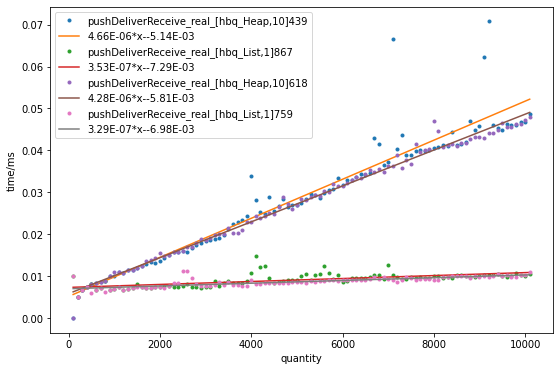
\includegraphics[scale=0.5]{Latex/Bilder/Plots/real_hbq_1_10.png}
\caption{\label{fig:real_heapListPercent} real - vgl. Heap, List (1\%,10\%)} 
\end{center}
\end{figure}

\newpage
Im letzten Plot (Abbildung \ref{fig:rand_heapListPercent}) wurden wieder die \textit{Delivery Queue} Limits parametrisiert. Statt 1\% und 10\% hier auf jeweils 10\% und 100\%. Gemessen wurden die zwei verschiedenen \textit{Holdback Queue} Strukturen mit zufällig sortierten Eingabelisten. Die Messungen bei 10\% sind wieder fast identisch und haben einen sehr flachen Verlauf. Bei 10000 Elementen dauert der Prozess 0,038ms pro Element. Die Messungen bei 100\% ergeben hingegen 0,175ms pro Element für den internen Heap und 0,225ms für die interne Liste. Die Differenz der beiden beträgt 0,05ms.

\begin{figure}[htbp]
\begin{center}
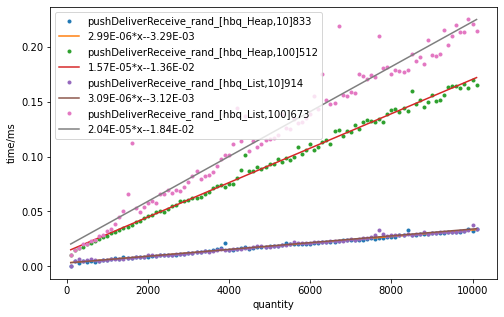
\includegraphics[scale=0.6]{Latex/Bilder/Plots/rand_heapList_10_100.png}
\caption{\label{fig:rand_heapListPercent} rand - vgl. Heap, List (10\%,100\%)} 
\end{center}
\end{figure}